\documentclass[a4paper, 18pt]{article}
\usepackage[T1]{fontenc}
\usepackage[utf8]{inputenc}
\usepackage[portuguese]{babel}
\usepackage[margin=3cm,includefoot,footskip=30pt]{geometry}

\usepackage{graphicx}
\graphicspath{ {imagens/} }
\usepackage{bold-extra}
\usepackage{epstopdf}
\usepackage{float}
\usepackage{scalerel}
\usepackage{enumerate}
\usepackage{indentfirst}
\usepackage{mathtools}
\usepackage{amsmath}
\allowdisplaybreaks
\usepackage{cleveref}
\usepackage{amssymb}
\usepackage{listings}
\usepackage{color}
\usepackage{textcomp}
\newcommand\showdiv[1]{\overline{\smash{\hstretch{.5}{)}\mkern-3.2mu\hstretch{.5}{)}}#1}}
\newcommand\ph[1]{\textcolor{white}{#1}}


\definecolor{dkgreen}{rgb}{0,0.6,0}
\definecolor{gray}{rgb}{0.5,0.5,0.5}
\definecolor{mauve}{rgb}{0.58,0,0.82}
\definecolor{mygreen}{RGB}{28,172,0} % color values Red, Green, Blue
\definecolor{mylilas}{RGB}{170,55,241}

% ----- Cabeçalho e rodapé -----
\usepackage{fancyhdr}
\pagestyle{fancy}
\fancyhf{}

\renewcommand{\headrulewidth}{1pt}
\renewcommand{\footrulewidth}{0.5pt}

\rhead{Word Morph}
\lhead{Algoritmos e Estruturas de Dados\rightmark}
\rfoot{Página \thepage}
\lfoot{\small Engenharia Eletrotécnica e de Computadores - IST}


\usepackage{pdfpages}

\begin{document}

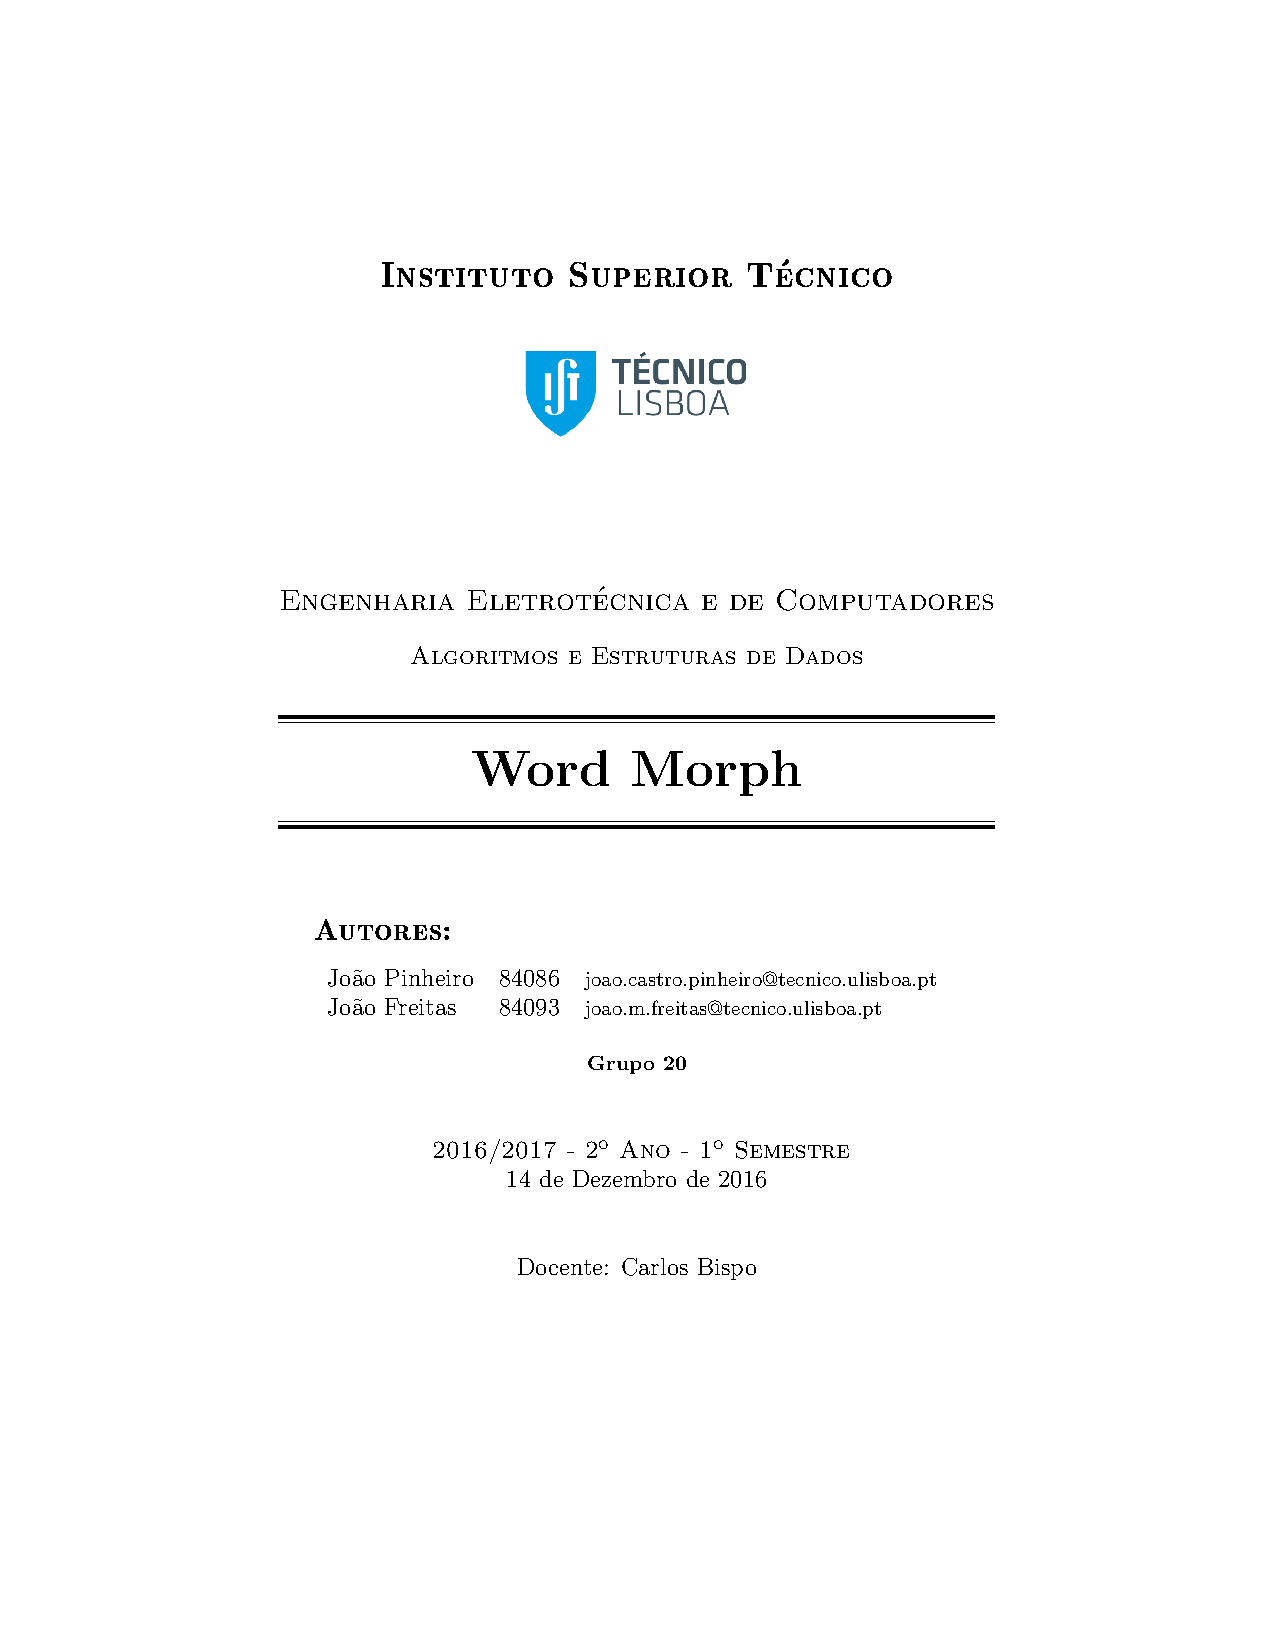
\includepdf[pages={1}]{capa/capa.pdf}

\tableofcontents
\newpage

\section{Especificação do problema}
	\par
	O problema proposto é encontrar caminhos entre duas palavras do mesmo tamanho. Estes caminhos consistem em permutações de letras. Em cada passo podem-se alterar no máximo um dado número de letras. No entanto, o peso duma ligação é o quadrado do número de carateres mudados. O objetivo é então encontrar o caminho de menor custo (i.e., que minimiza o peso total das ligações do caminho) entre a palavra de origem e a palavra de destino, passando por palavras do dicionário dado. Por exemplo, dado o problema:
	\begin{center}
		\texttt{dragar oravam 2}
	\end{center}
	\par
	É preciso encontrar o caminho de \textbf{dragar} a \textbf{oravam}, permutando, no máximo, 2 palavras em cada passo. Um caminho válido é então:
	\begin{center}
		\textbf{dragar} \\
		tragam \\
		\textbf{oravam}
	\end{center}
	\par
	Através de duas mutações de dois carateres cada. O custo total deste caminho é $2 \times 2^2 = 8$. No entanto, um caminho de menor custo seria:
	\begin{center}
		\textbf{dragar} \\
		tragar \\
		tragam \\
		travam \\
		\textbf{oravam}
	\end{center}
	\par
	Através de 4 mutações de um carater cada. O custo total deste caminho é $4 \times 1^1 = 4$, sendo de menor custo do que o anterior e, deste modo, a resposta correta.
	\par
	Para resolver grandes quantidades destes problemas, implementou-se uma solução na linguagem \textit{C}.
	O programa recebe dois parâmetros: \\
	\begin{itemize}
		\item Um ficheiro de dicionário de extensão \texttt{.dic} de palavras não acentuadas, não hifenadas e não necessariamente ordenado alfabeticamente, no formato de palavras separadas por um só espaço e uma ou mais palavras por linha.
		\item Um ficheiro de problemas de extensão \texttt{.pal} com vários problemas, um por linha, no formato:
		\begin{center}
		\texttt{<origem> <destino> <número máximo de permutações>}
		\end{center}
		\par
		Onde se assume que o formato está correto e as palavras pertencem ao dicionário.
	\end{itemize}
	\par
	O programa é invocado então da seguinte maneira:
	\begin{center}
		\texttt{\$ ./wordmorph <dicionário.dic> <problemas.pal>}
	\end{center}
	\par
	O programa escreve um ficheiro de saída de extensão \texttt{.path}, explicitando os caminhos e o custo associado, no seguinte formato, por exemplo, para o exemplo anterior \texttt{dragar oravam 2}:
	\begin{center}
		\texttt{
		dragar 4\\
		tragar \\
		tragam \\
		travam \\
		oravam}
	\end{center}
	\par
	É de notar que se não existir caminho, o peso será \texttt{-1}; se as palavras forem iguais, o peso será \texttt{0}. Existe uma linha em branco entre cada solução.


\section{Abordagem ao problema}
	\par
	Este problema é muito facilmente transposto num problema de grafos ponderados, em que os vértices representam palavras e as arestas ligações de $k$ permutações, sendo o peso da aresta igual a $k^2$.
	\par
	Como podem existir vários tamanhos de palavras no ficheiro de problemas, decidiu-se utilizar uma tabela de grafos indexada por um inteiro representando o tamanho de palavra que um grafo contém. Para construir os vários grafos, lê-se o ficheiro de problemas para perceber quais tamanhos de palavras e o respetivo número máximo de permutações seriam necessários. De seguida, criam-se as arestas no de acordo com este número, comparando palavra a palavra. Para resolver os problemas, utiliza-se um algoritmo de caminho mais curto no grafo pertinente.


\section{Arquitetura}
	<fluxogramas>
• Uma descrição completa da arquitectura do programa, incluindo fluxogramas
detalhados e um texto claro, mas sucinto, indicando a divisão lógica e funcional dos
módulos desenvolvidos para a resolução do problema, explicitando os respectivos
objectivos, as funções utilizadas e as estruturas de dados de suporte;

\section{Tipos de dados}
	- graph (vertex, edge)
	- heap
• Uma descrição detalhada dos tipos de dados utilizadas e justificação dos mesmos
(tabelas, listas, filas, pilhas, árvores, grafos, acervos, etc.);

\section{Algoritmos}
	- dijkstra
	- g\textunderscore make\textunderscore edges
	- fprint\textunderscore path
• Descrição dos algoritmos usados (por exemplo, na manipulação dos tipos de dados);

\section{Subsistemas}
	- file.c
	- heap.c
	- graph.c
	- dijkstra.c
	- word.c
• Uma descrição dos subsistemas funcionais que existam e, para cada um:
	– a descrição dos objectivos do subsistema (até 5 linhas);
	– o nome do módulo onde estão definidos os tipos de dados abstractos
	  (ficheiros .h) a utilizar no subsistema;
	– o nome do módulo C onde estão as funções do respectivo subsistema;
	– listagem das funções implementadas no subsistema, indicando para cada uma a
	  respectiva assinatura e os objectivos da função (descrição sumária, sem código);

\section{Análise de complexidade}
	- fors do file.c $O(n)$
	- dijkstra $\Theta((E+V) lg V)$
	- g\textunderscore make\textunderscore edges $O(V^2)$
	- memoria: $\Theta(V + E)$
• Uma análise, formal e/ou empírica, dos requisitos computacionais do programa desenvolvido, tanto em termos da memória que utiliza como da complexidade computacional, com particular ênfase no custo das operações de processamento sobre os tipos de dados usados e/ou criados;

\section{Análise crítica}
• Uma análise crítica do funcionamento do programa e a avaliação do desempenho
do projecto implementado;

\section{Exemplo de execução}
	\par
	Por exemplo, para o ficheiro de problemas:
	\begin{center}
		\texttt{tragar travam 2}
	\end{center}
	\par
	E para o dicionário:
	\begin{center}
		\texttt{tragar tragam travam a flores}
	\end{center}
	\par
	Depois de verificar os parâmetros de entrada e abrir os ficheiros, \texttt{find\textunderscore max\textunderscore perms()} é chamada.
	Inicializa \texttt{max\textunderscore perms} a zero e de seguida o ficheiro de problemas é lido: como \texttt{w\textunderscore diff()} devolve 2 e \texttt{max\textunderscore perms[6] = 0 < 2}, então \texttt{max\textunderscore perms[6] = 2} e os restantes índices ficam iguais a zero.
	\par
	A seguir constrói-se o grafo, chamando \texttt{read\textunderscore dic()}. Esta função primeiramente lê o dicionário à procura do número de palavras de cada tamanho a alocar, e chega a \texttt{num\textunderscore words[6] = 4} pois \texttt{max\textunderscore perms[1] = max\textunderscore perms[5] = 0}. Seguidamente, \texttt{graphs[6]} é inicializado com 4 vértices (palavras), ficando os restantes valores nos índices \texttt{i} de \texttt{graphs} iguais a \texttt{NULL} pois representam os restantes tamanhos de palavra em que \texttt{max\textunderscore perms = 0}. Agora o dicionário é lido outra vez para alocar as palavras em si, sendo \texttt{g\textunderscore insert()} e \texttt{w\textunderscore new()} chamadas 4 vezes, correspondendo às 4 palavras de tamanho 6. A seguir é chamada \texttt{g\textunderscore make\textunderscore edges()} para construir as arestas entre os vértices do grafo de tamanho de palavra 6. A tabela de vértices é:
	\texttt{[0: "tragar", 1: "tragam", 2: "travam", 3: "flores"]}
	\par
	Os resultados dos ciclos são apresentados de seguida:
	\begin{itemize}
		\item
			\texttt{i = 0, j = 0} \\
			\texttt{---------------------}
		\item
			\texttt{i = 1, j = 0} \\
			\texttt{calc\textunderscore weight("tragam", "tragar", 2) = 1} \\
			\texttt{e\textunderscore add(g, 1 ("tragam"), 0 ("tragar"), 1)}
		\item
			\texttt{i = 2, j = 0} \\
			\texttt{calc\textunderscore weight("travam", "tragar", 2) = 2} \\
			\texttt{e\textunderscore add(g, 2 ("travam"), 0 ("tragar"), 4)}
		\item
			\texttt{i = 2, j = 1} \\
			\texttt{calc\textunderscore weight("travam", "tragam", 2) = 1} \\
			\texttt{e\textunderscore add(g, 2 ("travam"), 1 ("tragam"), 1)}
		\item
			\texttt{i = 3, j = 0} \\
			\texttt{calc\textunderscore weight("flores", "tragar", 2) = 3}
		\item
			\texttt{i = 3, j = 1} \\
			\texttt{calc\textunderscore weight("flores", "tragam", 2) = 3}
		\item
			\texttt{i = 3, j = 2} \\
			\texttt{calc\textunderscore weight("flores", "travam", 2) = 3}
	\end{itemize}
	\par
	O grafo resultante em forma gráfica:
	% TODO: pls freitas halp
	\begin{figure}[h]
		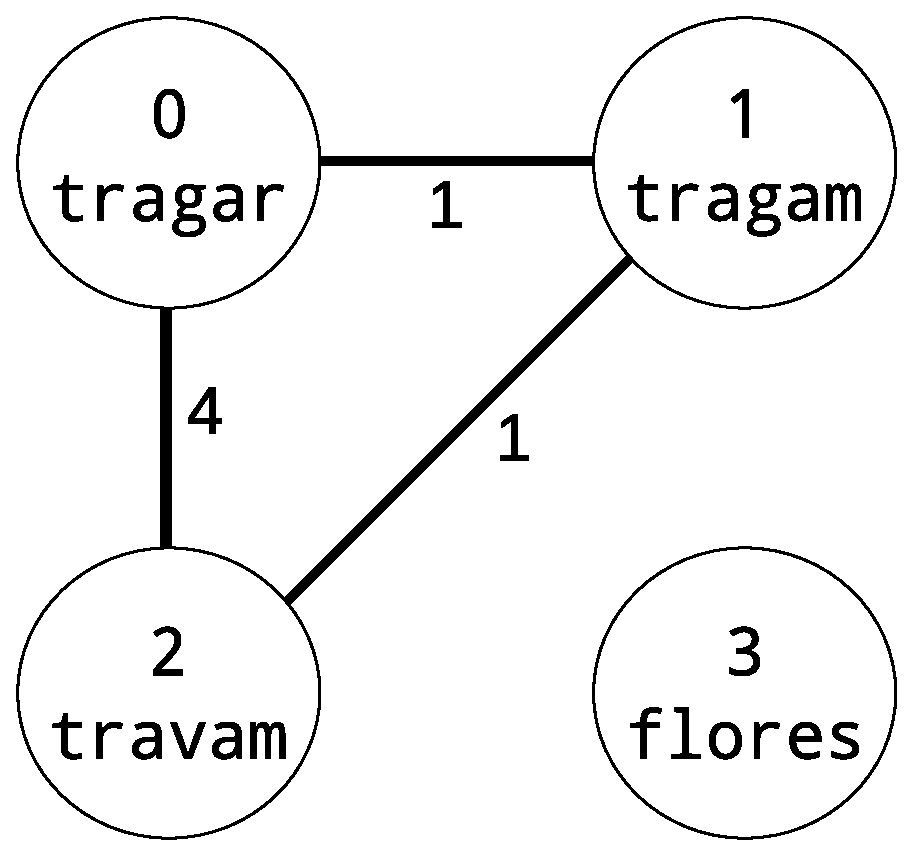
\includegraphics[width=0.5\linewidth]{graph}
	\end{figure}
	\par
	E o grafo resultante como representado no programa, sob listas de adjacências: \\
	\begin{center}
		\texttt{0: 1 \textrightarrow{} 2 \textrightarrow{} NULL \\
				1: 0 \textrightarrow{} 2 \textrightarrow{} NULL \\
				2: 0 \textrightarrow{} 1 \textrightarrow{} NULL \\
				3: \textrightarrow{} NULL}
	\end{center}

		\textbf{dragar} \\
		tragar \\
		tragam \\
		travam \\
		\textbf{oravam}


• Pelo menos, um pequeno exemplo completo e detalhado de aplicação, com descrição
da utilização das estruturas de dados em cada passo e de como são tomadas as
decisões.

\end{document}
